\documentclass[4apaper]{report}
\usepackage{graphicx}
\usepackage[utf8]{inputenc}
\usepackage[portuguese]{babel}
\usepackage{a4wide}
\title{Projeto de Laboratórios de Informática 1\\Grupo 135}
\author{José André Martins Pereira a82880 \and André da Costa Almeida a82046}
\date{\today}

\begin{document}
\maketitle
\begin{abstract}
Este Relatório desenvolvido na Unidade Curricular de Laboratórios de Informática 1, da Licenciatura em Engenharia Informática da Universidade do Minho, apresenta a elaboração do jogo Bomberman, usando a linguagem de programação funcional Haskell.
\end{abstract}
\tableofcontents

\section{Introdução}
\label{sec:intro}

No âmbito da Unidade Curricular de Laboratórios de Informática I (LI1), da Licenciatura em Engenharia Informática da Universidade do Minho, foi nos proposta a elaboração de um projeto, o jogo clássico Bomberman. 

O trabalho foi dívidido em duas fases. Na primeira fase tratou-se da geração de mapas, compressão, descompressão dos mesmos e da reação a comandos do utilizador. 

A segunda fase do projecto, teve como objetivo a passagem do tempo, em especial atenção na explosão das bombas e a respetiva destruição. Foi elaborada uma interface gráfica do jogo, onde conjugou-se os subprogramas da primeira fase e da segunda, com a finalidade de conseguir um aspeto e jogabilidade, semelhante ao clássico. Por fim, na segunda fase, foi criado um \textbf{Bot}, ou seja, um simulador de ações humanas, que neste caso, será um adversário com uma inteligência arteficial, capaz de jogar contra o utilizador.

\section{Descrição do Problema}
\label{sec:approjecto}

O objetivo principal a atingir neste projeto é desenvolver um jogo semelhante ao clássico Bomberman, ou seja, uma interface gráfica idêntica, e a mesma jogabilidade.

\section{Primeira fase do Projeto}
\label{sec:primeirafase}

\subsection{Primeira Tarefa}

A primeira Tarefa tem como objetivo a geração de mapas pseudo aleatórios, usando o tamanho\footnote{O tamanho corresponde á largura do mapa, sendo que o tabuleiro do jogo é sempre quadrado (o tamanho é sempre número ímpar, superior ou igual a 5).} e semente\footnote{A semente é utilizada para que haja diferentes mapas com o mesmo tamanho.} dos mesmos. 

O mapa ou tabuleiro é uma grelha quadrada em que cada célula pode ser vazia, conter um bloco de pedra indestrutível ou um bloco de tijolo destrutível por uma bomba. Alguns blocos de tijolo podem esconder power ups, que servem para aumentar a capacidade do jogador.

Observando esta estrutura foi criada uma função capaz de gerar números aleatórios num determinado intrevalo, mas tal como foi dito anteriormente esta aleatoriedade é pseudo, pois para a mesma semente, são gerados sempre os mesmos números, assim é possível jogar diferentes mapas com o mesmo tamanho, mas com conteúdo diferente, devido à semente. 

Após gerada a lista de números aleatórios inteiros e através da Tabela de Conteúdo (Tabela 1), criou-se uma função, que se pode ver abaixo que converte a lista de números, para a lista dos respetivos carateres. A utilidade desta lista é preencher as células que irão ter conteúdo variado (Tijolos,Power Ups,Células Vazias).

\begin{verbatim}
determina_Char :: [Int] -> [Char]
determina_Char [] = [] 
determina_Char (h:t) | h >= 0 && h <= 1 = '+':determina_Char t 
                     | h >= 2 && h <= 3 = '!':determina_Char t 
                     | h >= 4 && h <= 39 = '?':determina_Char t 
                     | h >= 40 && h <= 99 = ' ':determina_Char t
\end{verbatim}

\begin{table}[ht]
\centering
\begin{tabular}[t]{|l|l|c|}\hline
	Gama & Conteúdo & Caracter \\\hline
	0 a 1 & Power up Bombs escondido atrás de um tijolo. & '+'\\\hline
	2 a 3 & Power up Flame escondido atrás de um tijolo. & '!'\\\hline
	4 a 39 & Tijolo. & '?' \\\hline
	40 a 99 & Vazio. & ' '\\\hline
	\end{tabular}
	\caption{Tabela de Conteúdo.}
	\label{table:tabConteudo}
\end{table}


Tal como se pode observar na (Figura 1), de um mapa do jogo Bomberman, este é constituído por paredes laterais, superior e inferior, contém ainda linhas com células vazias e tijolos, portanto sem pedras, designadas por linhas sem pilares, outras linhas em que existem pedras intercaladas e tijolos colocados aleatoriamente, denominadas por linhas com pilares. 

\begin{figure}[ht]
	\centering
	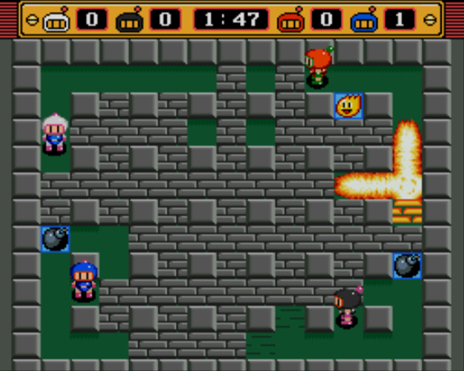
\includegraphics[scale=1.5]{tabuleiro.jpg}
	\caption{Mapa Bomberman}
	\label{img:mapa}
\end{figure}

A estratégia utilizada para a construção do tabuleiro do jogo foi através da paridade das posições das linhas, ou seja, observando o mapa (Figura 1), verifica-se que as linhas sem pilares, ocorrem nas posições ímpares (tendo em conta que a primeira posição é zero), enquanto que as linhas com pilares ocorrem nas posições pares. Logo, através desta característica conseguiu-se gerar um mapa semelhante ao do Bomberman. 

Posteriormente foram desenvolvidas funções que desenham os diferentes tipos de linhas que existem no tabuleiro, acrescentando ainda os caracteres especiais (Tijolos, Power Ups, células vazias), nas células de conteúdo variado, analisadas anteriormente. Como foi dito inicialmente, existem Power Ups escondidos atrás de tijolos, portanto foi necessário guardar as posições em que eles ocorrem, por isso, quando o caracter do conteúdo aleatório é um power up, as coordenadas dele são guardadas.

\subsection{Testes da Primeira Tarefa}
O método de testes da Primeira Tarefa, foi testar a geração de mapas com tamanho aleatório, e verificar se esses mapas correspondiam ao esperado.

\subsection{Segunda Tarefa}
A segunda Tarefa tem como objetivo, a reação a comandos do utilizador, ou seja, receber um estado de jogo, um comando, e verificar quais as alterações com o respetivo comando.

Analisando o jogo original, verifica-se que os comandos existentes são os direcionais e a colocação de bombas.  Assim as alterações possíveis na informação do mapa serão a ativação de bombas, o movimento do jogador e a possível capturação de power ups. Portanto é necessário atualizar a informação das coordenadas do jogador e caso este tenha apanhado um power up, será necessário elimina-lo da informação do mapa e acrescentá-lo à informação do jogador.

Os primeiros passos para a concretização do objetivo desta Tarefa foi trabalhar sobre os comandos direcionais. Assim, começou-se por verificar se o comando recebido é uma jogada válida, para averiguar, testa-se se na posição para onde o jogador pertende ir, existe algum bloco que não permita a sua passagem, ou seja, se existe uma pedra ou um tijolo a bloquear o caminho. 

No caso do comando da ativação da bomba, a validação deste passa por, confirmar se já existe alguma bomba na posição e se o jogador, tem bombas para colocar. Após a validação da jogada, determina-se quais as possíveis alterações na informação do mapa. 

Caso o comando seja direcional, as mudanças do estado de jogo, são a atualização das coordenadas da informação do jogador e a possível captura de power ups, neste último caso, é necessário, eliminar a informação do power up, e acrecentar o respetivo, à informação do jogador. 

Pode-se ver a seguir a função principal da segunda Tarefa, onde é vísível, a ordem de acontecimentos, ou seja, inicialmente testa-se se a jogada é válida e depois caso seja, verifica-se as alterações causadas no mapa pelo comando, caso contrário retorna-se o mapa recebido. O primeiro caso da função resulta na situação de o jogador estar morto, e assim a função \textbf{detposjogador} retorna a posição (0,0), logo retornamos o mapa inicial.

\begin{verbatim}
move :: [String] -> Int -> Char -> [String]  
move mapa gamer cmd | c == 0 && l == 0 = mapa 
				    | validar_comando mapa cmd gamer (c,l) = 
				    	det_mapa_res mapa cmd gamer c_cmd l_cmd 
				    | otherwise = mapa 
				        where (c,l) = det_pos_jogador mapa gamer
				              (c_cmd,l_cmd) = determina_pos cmd (c,l)
\end{verbatim}

No caso, de colocação de bombas, as alterações passam por acrescentar a informação da mesma ao mapa, por isso, é necessário saber qual é o jogador que a está a colocar, verificar os seus power ups flames, para saber qual o raio de ação da bomba, e assim colocá-la na informação do mapa.

O próximo exemplo, representa a utilização da função da Segunda Tarefa, aplicada a um situação de jogo, onde se observa dois jogadores, uma bomba ativada pelo jogador 1, com raio 1, e o jogador 0 já capturou um power up Bomb.

\begin{verbatim}

#########
#       #
# #?# # #
#     ? #
#?# # #?#
# ?  ?  #
# #?#?# #
#  ??   #
#########
+ 3 3
! 5 5
* 7 7 1 1 10
0 4 3 +
1 7 7
\end{verbatim}

O jogador 1 fez o comando 'L', ou seja, para a esquerda e apanhou o power up Bomb na posição 3 3.

\begin{verbatim}
#########
#       #
# #?# # #
#     ? #
#?# # #?#
# ?  ?  #
# #?#?# #
#  ??   #
#########
! 5 5
* 7 7 1 1 10
0 3 3 ++
1 7 7

\end{verbatim}

As principais difículdades encontradas nesta Tarefa, foi a manipulação de Strings, visto que, precisamos de remover e acrescentar informação do mapa que está no tipo \textbf{[String]}, para ultrapassar esta dificuldade, foram utilizadas funções predefinidas de manipulação de Strings, tal como (\textbf{unwords,words,unlines,etc...}).

\subsection {Testes da Segunda Tarefa}
Os testes utilizados para a verificação da Segunda Tarefa, foi principalmente a validação de comandos, por exemplo colocar uma bomba e um jogador na mesma posição para testar se esse jogador consegue ativar bombas. Do mesmo modo, averigou-se se o jogadores tentavam passar por cima de tijolos e pedras. Igualmente, testou-se a captura de power ups, por parte dos jogadores.

\subsection{Terceira Tarefa}
A Terceira Tarefa tem como objetivo a compressão e descompressão do mapa, ou seja, tentar utilizar o menor número de caracteres possível de forma que não seja perdida informação do jogo e que seja possível através de uma descompressão voltar a ter o mapa inicial.

Inicialmente, observando o mapa, verifica-se que existe muito conteúdo que é constante em todos os mapas, portanto, começou-se por eliminá-lo, ou seja, remover as pedras. Mas para não se perder informação, guardou-se o tamanho do mapa no ínicio da String, comprimindo este também, utilizando para isso as posições dos caracteres da tabela \textbf{ASCII}, substituindo este por um caracter, portanto, o tamanho corresponde à posição deste caracter na Tabela \textbf{ASCII}. 

Após a remoção das pedras, verificou-se a existência de algo que não é igual em todos os mapas, mas que era possível otimizar, os espaços vazios, a ideia é substituir os espaços vazios consecutivos, pelo número de espaços, por exemplo: 5 espaços seguidos vazios são substituidos pelo caracter '5', e assim temos a compressão de 5 caracters em 1.

No próximo exemplo podemos ver a compressão e descompressão do mapa com tamanho 11 e semente 0, o \textbf{encode}, faz a compressão do mapa, removendo as pedras e substituindo os espaços vazios pelo seu número.

Por outro lado, o \textbf{decode} faz a descompressão do mapa comprimido, ou seja, coloca as pedras removidas, e substitui os números por espaços. 

\begin{figure}[ht]
	\centering
	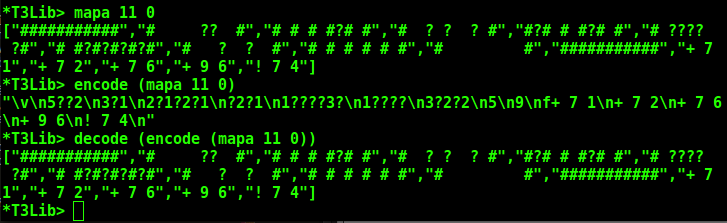
\includegraphics[scale=0.75]{terminalT3.jpg}
	\caption{Utilização das Funções da Terceira Tarefa (\textbf{encode, decode}).}
	\label{img:terminaT3}
\end{figure}

\begin{itemize}
	\item A função \textbf{mapa}, está definida na Primeira Tarefa, é usada para geração de mapas.
\end{itemize}

Existiam outras metas a atingir nesta Tarefa, como substituir as coordenadas dos power ups por caracteres da Tabela \textbf{ASCII}, mas não houve possíbilidade, pois certos mapas não eram bem comprimidos, porque quando o número das coordenadas era superior a 47 e inferior a 58, ocorriam erros, pois os caracteres destas posições correspondem aos números de 0 a 9. 

%Para a realização da descompressão do mapa comprimido recorreu-se à compressão, ou seja, se na compressão 
%
\subsection{Testes da Terceira Tarefa}
O método utilizado para testar esta Tarefa foi a compressão e descompressão de diferentes mapas, em que o resultado final esperado será o mapa inicial. Utilizou-se diferentes mapas, com pequenas e grandes dimenssões, com vários power ups, de forma a tentar testar o maior número de possibilidades.

\section{Segunda fase Projecto}
\label{sec:segundafase}

\subsection{Estrutura de Dados: Quarta Tarefa}
Com o henriquecimento de conteúdo acerca da linguagem funcional Haskell ao longo do semestre, aplicou-se nesta Tarefa tipos de dados novos, de modo, a facilitar a manipulação de dados, ou seja, a informação do mapa, que se torna díficil com \textbf{Strings}. Para isso criou-se um data chamado \textbf{Bloco}, que contém os construtores \textbf{Pedra, Tijolo e Vazio}, que são os diferentes tipos de blocos do \textbf{Tabuleiro}. 

\begin{verbatim}
data Bloco = Pedra 
           | Tijolo 
           | Vazio 
        deriving (Show,Eq)
\end{verbatim}

De seguida, criou-se um novo tipo para os power ups, denominado por \textbf{PowUp}, com os construtores, \textbf{Bomb e Flame}, e as respetivas posições, \textbf{type Posicao = (Int,Int)}, destes. 

\begin{verbatim}
type Posicao = (Int,Int)
data PowUp = Bomb Posicao | Flame Posicao 
        deriving Show
\end{verbatim}

Por fim, e não menos importante, criou-se o tipo \textbf{Player}, em que os seus construtores, facilitaram bastante o trabalho de remoção e adição de informação, que são \textbf{Vivo e Morto}, em que no construtor \textbf{Vivo}, ainda temos a sua posição, através do \textbf{type Posicao = (Int,Int)}, número de power ups bombs e flames, utilizando \textbf{type NumbFlame = Int, type NumbBomb = Int}. 

\begin{verbatim}
type Posicao = (Int,Int)
type NumbBomb = Int
type NumbFlame = Int
data Player = Vivo Posicao NumbBomb NumbFlame
            | Morto
        deriving (Show,Eq)
\end{verbatim}

\subsection{Quarta Tarefa}

A quarta Tarefa tem como objectivo, verificar as alterações, causadas pela passagem do tempo.

% logo incide na explosão das bombas e a destruição que estas causam, que pode ser a morte de jogadores, destruição de tijolos ou power ups.
%

Começou-se por analisar, quais as alterações significativas, assim, verificou-se que o principal foco será as bombas, principalmente a destruição que causam. Portanto, o primeiro passo, foi identificar se existem bombas que vão explodir no instante de tempo em que a função é chamada. 

Definiu-se que as Bombas explodem, quando o seu tempo é igual a um, portanto começou-se por separar as bombas que vão explodir, das que não vão explodir neste instante de tempo. Depois, determinou-se o range de explosão de cada bomba, sendo que o flame das bombas não ultrapassa pedras, tijolos e power ups, mas no caso dos tijolos e power ups, estes são destruídos. Para isso definiu-se uma função que determina as posições do range de cada bomba, a qual podemos ver abaixo.

\begin{verbatim}
detRangeCoords :: Bomba -> Int -> InfGame -> [Posicao]
detRangeCoords ((c,l),j,f,t) size infgame = 
  (c,l):(direction ((c,l-1),j,f,t) f size infgame Cima )++
  (direction ((c,l+1),j,f,t) f size infgame Baixo)++
  (direction ((c-1,l),j,f,t) f size infgame Esquerda)++
  (direction ((c+1,l),j,f,t) f size infgame Direita)
   where 
          direction ((c,l),j,f,t) rangeFlame size infgame dir 
            | rangeFlame <= 0 = []
            | blc == Pedra && rangeFlame > 0 = []
            | blc == Tijolo && rangeFlame > 0 = (c,l):[] 
            | exist = (c,l):[]
            | rangeFlame > 0 = 
            	(c,l):(direction ((detCoords dir (c,l)),j,f,t) (rangeFlame-1) size infgame dir)
            | otherwise = []
              where blc = bloco infgame (c,l) 
                    (exist,pwUps) = checkPosPowerUp p (c,l)
                    p = powerUps infgame
\end{verbatim}

Como se pode ver na função, esta verifica as quatro direções possíveis do range da \textbf{Bomba}, visto que a função \textbf{direction}, determina através da direção (\textbf{Cima, Baixo, Esquerda e Direita}), quais as posições da explosão de uma bomba, até ao range máximo do flame. 

Inicialmente verifica-se se o \textbf{rangeFlame} já terminou, ou seja, se é menor ou igual a zero, depois, caso o flame ainda não tenha terminado, averigua-se se o bloco é um pedra, retornando, assim, lista vazia, pois não se destroi as pedras. 

Se o bloco não for uma pedra, tem que se testar se é um tijolo, sendo este caso diferente do anterior, pois o tijolo é destrutível, por isso, necessita-se de retornar a sua posição. 

Do mesmo modo, se existir um power up na posição indicada, retornamo-la, para que ele seja destruído, mas não se retorna mais nada, pois o flame não ultrapassa, power ups.

Por fim, se não for nenhum dos casos anteriormente descritos, é o caso normal, ou seja, não existe nada a impedir a passagem do flame e simplesmente, retorna-se a posição atual e continua-se a testar as próximas através da recursividade.

Ainda na Quarta Tarefa, foi realizada um função que desenha uma espiral no mapa com o bloco \textbf{Pedra}, que é característica do clássico jogo \textbf{Bomberman}, a utilidade desta é obrigar os jogadores a morrerem para sobreviver apenas um e ser o vencedor. 

Para a elaboração deste algoritmo foi necessário, visualizar a espiral e identificar as posições onde ocorrem as pedras. Assim foi feita uma função chamada \textbf{posSpiral}, que se pode ver abaixo, capaz de retornar todas as posições da espiral de qualquer mapa, ou seja, as posições onde tem que se colocar uma pedra em cada instante de tempo. 

\begin{verbatim}
posSpiral :: Size -> [Posicao]
posSpiral size = aux_posSpiral (1,1) size 0 2 
aux_posSpiral (c,l) size flag prof
  | c == (size `div` 2) && l == (size `div` 2) = (c,l):[]
  | flag == 0 && c == (size-prof) = (c,l):(aux_posSpiral (c,l+1) size 1 prof)
  | flag == 0 = (c,l):aux_posSpiral (c+1,l) size flag prof
  | flag == 1 && l == (size-prof) = (c,l):(aux_posSpiral (c-1,l) size 2 prof)  
  | flag == 1 = (c,l):aux_posSpiral (c,l+1) size flag prof
  | flag == 2 && c == (prof-1) = (c,l):(aux_posSpiral (c,l-1) size 3 prof)
  | flag == 2 = (c,l):aux_posSpiral (c-1,l) size flag prof
  | flag == 3 && l == (prof-1) = aux_posSpiral (c+1,l+1) size 0 (prof+1)
  | flag == 3 = (c,l):(aux_posSpiral (c,l-1) size flag prof)
\end{verbatim}

Observando, a lista de posições, verifica-se que qualquer espiral começa na posição (1,1). O parâmetro \textbf{prof}, corresponde à profundidade de cada anel da espiral no mapa, sendo o seu valor inicial 2, mas logicamente a profundidade deveria ser 1, mas devido às posições começarem em zero, a profundida é igual a 2. As \textbf{Flags}, são zero, um, dois, três, que na verdade correspondem à pareda superior, lateral direita, inferior e lateral esquerda, respetivamente, portanto, elas servem apenas para saber em que momento a espiral se encontra. 

Quando a espiral está nas linhas superiores, ao longo destas as posições onde vão cair as pedras variam no incremento da coluna. A espiral na parede superior termina quando a coluna é igual a \textbf{(size\footnote{O parâmetro \textbf{size}, corresponde ao tamanho do mapa, que se falou anteriormente.}-prof)}. Depois quando a linha for igual a \textbf{(size-prof)} significa que estamos no fim da parede lateral direita, e ao longo desta, incrementou-se a linha das posições onde devem cair as pedras, e passa-se para a parede inferior, que acaba quando a coluna for igual a \textbf{(prof-1)}, e ao longo desta parede, decrementa-se a coluna das posições onde devem cair as pedras. 

Por fim, o primeiro anel da espiral termina na parede lateral esquerda, quando a linha for igual a \textbf{(prof-1)}, ao longo desta parede as posições das pedras variam com o decremento da linha. No fim desta última parede incrementa-se a profundidade para desenhar as posições do próximo anel da espiral. 

Depois de gerada a lista de posições da espiral, necessita-se de saber em que posição tem que cair a pedra, para colocá-la.  

\subsection{Testes da Quarta Tarefa}
Os testes utilizados, para testar a Quarta Tarefa, basearam-se na explosão das \textbf{Bombas}, por isso, colocou-se bombas próximas de tijolos, power ups, jogadores, pedras, de outra bombas, verificou-se também a explosão de várias \textbf{Bombas} em simultâneo, para conseguir testar ao máximo a Quarta Tarefa. 

Para testar o efeito espiral e os testes que foram referidos anteriormente, utilizou-se também a interface gráfica, elaborada na Quinta Tarefa.

\subsection{Estrutura de Dados: Quinta Tarefa}
Os tipos de dados utilizados na Quinta Tarefa, foram os mesmo que na anterior, visto que, facilitam muito a extração de informação do mapa. Mas houve a necessidade de ser criado um novo tipo de dados denominado por \textbf{Imagens}, com o objetivo de carregar e guardar as imagens que são utilizadas na interface gráfica, usando um record, pode-se observar este novo tipo de dado abaixo.

\begin{verbatim}
data Imagens = Imagens { pedra :: Picture,
                         bomba :: Picture, 
                         caixa :: Picture, 
                         jogador0 :: Picture, 
                         jogador1 :: Picture, 
                         jogador2 :: Picture, 
                         jogador3 :: Picture, 
                         powUpBomb :: Picture, 
                         powUpFlame :: Picture, 
                         fundo :: Picture, 
                         explosion :: Picture}
\end{verbatim} 

\subsection{Quinta Tarefa}

A Quinta Tarefa tem como objetivo, o desenvolvimento de uma interface gráfica, para o jogo e conjugar todas as funções anteriormente criadas de modo a conseguir que esta seja jogada, para a concretização deste objetivo foi utilizada a biblioteca \textbf{Gloss}.

Inicialmente, definiu-se, quantos elementos tem o \textbf{Estado de Jogo}, ou seja, a informação necessária para as funções, necessitou-se da informação do mapa, do tamanho e semente do mesmo, posteriormente, precisou-se do somatório de (\textbf{1/Frame Rate}), as imagens utilizadas na interface gráfica, o tempo atual do jogo, a largura e altura em píxeis do mapa e por fim o número do jogador, tal como pode-se ver abaixo.
.
\begin{verbatim}
type Estado = (InfGame,
			  Tamanho,
			  Semente,
			  LastTimeReageT,
			  Imagens,
			  ActualTime,
			  WindowLargura,
			  WindowAltura,
			  Gamer)
\end{verbatim}  

Após a definição do \textbf{Estado de Jogo}, necessita-se de criar um estado inicial, ou seja, "carregar" o \textbf{Estado de Jogo}, então utilizando a class \textbf{Monad}, pede-se ao utilizador para escolher o tamanho, semente e jogador. 

Assim consegue-se gerar o conteúdo inicial, criando o \textbf{Tabuleiro}, através da função \textbf{mapa} definida na \textbf{Primeira Tarefa}, o somatório de (\textbf{1/Fram Rate}) é inicializado a zero, as imagens são guardadas no record do tipo \textbf{Imagens}, o tempo atual do jogo é inicializado com duas vezes o número de blocos interiores do mapa, a largura e altura do \textbf{Tabuleiro}, é o produto do tamanho por 50 (cada imagem tem 50x50 píxeis) píxeis, e por fim o número do jogador.

Posteriormente, criou-se uma função, denominada \textbf{desenhaEstado}, capaz de criar qualquer estado de jogo numa imagem, para isso, dividiu-se as diferentes informações do mapa, e criou-se diferentes funções, em que cada uma retorna uma lista de imagens referentes à sua informação, depois a função \textbf{desenhaEstado} junta esta lista de imagens numa só. 

Inicialmente, criou-se a imagem do Tabuleiro, após esta, gerou-se a imagem dos power ups destapados, depois originou-se a imagem das bombas, por fim, e caso haja, desenhou-se o flame das bombas que explodem neste instante de tempo.

Com a função \textbf{desenhaEstado}, e conjugando as funções de outras Tarefas, consegue-se criar a interface gráfica. Como o utilizador necessita de comandos para mover o seu jogador, então criou-se uma função denominada \textbf{reageEvento}, que recebe o \textbf{Estado de Jogo} e uma tecla e retorna as alterações necessárias com o auxilio da função \textbf{move}, definida na Segunda Tarefa, que dado a informação do mapa, um comando, retorna o mapa com as alterações causadas pelo comando. Depois de recebido este mapa com as alterações, vai se atualizar a imagem da interface gráfica, com a função \textbf{desenhaEstado}, e assim sucessivamente.

Por fim, falta conjugar a passagem do tempo, às funções anteriores, desenvolvendo assim a função \textbf{reageTempo}, que utilizou a função \textbf{avanca}, definida na Quarta Tarefa, que retorna o mapa com as alterações, causadas pela passagem do tempo, como a explosão de bombas e os seus estragos. 

\begin{figure}[ht]
	\centering
	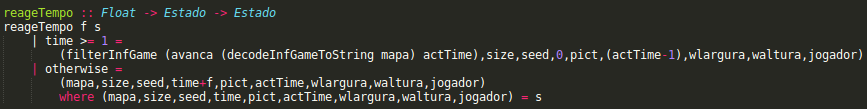
\includegraphics[scale=0.70]{algo_T5.jpg}
	\caption{Função \textbf{reageTempo}.}
	\label{img:algoT5}
\end{figure}

Como se pode ver a cima, a função \textbf{reageTempo}, recebe um parâmetro \textbf{f} e \textbf{s} que são (\textbf{1/Frame Rate}) e \textbf{Estado de Jogo}, respetivamente. Tal como foi visto anteriormente, no \textbf{Estado de Jogo}, existe um parâmetro denominado \textbf{LastTimeReageT}, que na verdade é o somatório de \textbf{f}, o qual é chamado nesta função de \textbf{time}, logo quando time é superior ou igual a um, significa que passou um segundo, logo pode-se chamar a função \textbf{avanca} e decrementar um unidade ao tempo atual de jogo \textbf{actTime}, caso contrário, significa que ainda não passou um segundo, logo retorna-se o estado recebido, atualizando o somatório de f, ou seja, (\textbf{1/Frame Rate}).

\begin{figure}[ht]
	\centering
	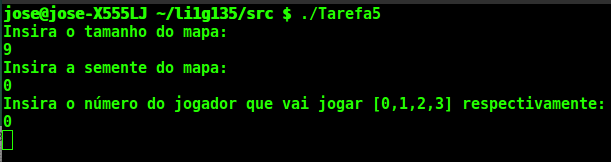
\includegraphics[scale=0.70]{monad.jpg}
	\caption{Input de Dados para o Estado Inicial.}
	\label{img1:monadT5}
\end{figure}

Conjungado todas estas funções, de todas as Tarefas, conseguiu-se ter um Interface Gráfica e jogabilidade semelhante ao clássico jogo Bomberman, essa conjugação é feita pela função \textbf{play}, predefinida na biblioteca Gloss. A imagem anterior e as seguintes são o resutado da Quinta Tarefa.

\begin{figure}[ht]
	\centering
	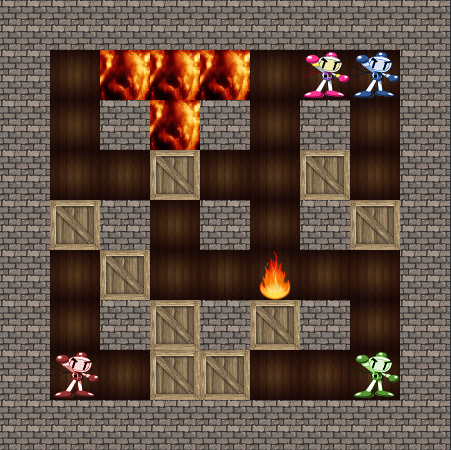
\includegraphics[scale=0.45]{1.jpg}
	\caption{Visualiza-se uma bomba a explodir e um power up flame destapado.}
	\label{img2:1T5}
\end{figure}

\begin{figure}[ht]
	\centering
	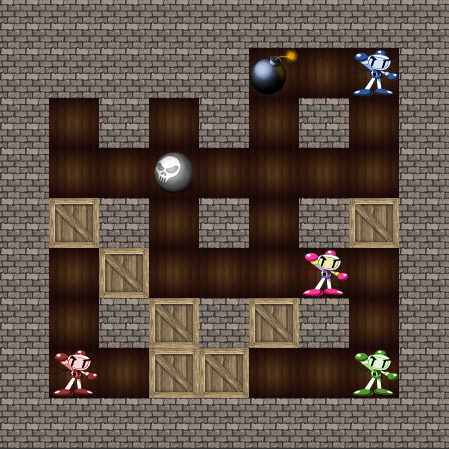
\includegraphics[scale=0.45]{2.jpg}
	\caption{Visualiza-se a espiral, um power up bomb destapado e uma bomba ativada.}
	\label{img3:2T5}
\end{figure}

\subsection{Estrutura de Dados: Sexta Tarefa}

Os tipos de dados utilizados na Sexta Tarefa, foram os mesmos que a Quarta Tarefa, mas criaram-se dois tipos novos, muito importantes no desenvolvimento desta. 

O primeiro tipo definido foi o \textbf{Dir}, como pode-se ver abaixo, que tem como objetivo, identificar as diferentes direções que o \textbf{Bot}, pode efetuar. 

O segundo tipo, foi \textbf{WhereIsBomb}, em que os seus construtores, indicam a localização de uma bomba ou a não existência dela, este tipo é muito importante, na fuga do \textbf{Bot} às \textbf{Bombas}.

\begin{verbatim}
data Dir = Upp | Downn | Leftt | Rightt | Null
    deriving (Show,Eq)

data WhereIsBomb = LinhaE | LinhaD | ColunaC | ColunaB | Bombspot | Nada
    deriving (Show,Eq)
\end{verbatim}

\subsection{Sexta Tarefa}

A sexta Tarefa tem como objetivo a criação de um \textbf{Bot}, ou seja, um simulador de ações humanas, que neste caso será um adversário com inteligência arteficial.

Inicialmente, o objetivo foi elaborar um \textbf{Bot}, capaz de fugir ao efeito espiral, mas com o decorrer do tempo, desenvolveu-se, um \textbf{Bot}, capaz de perseguir e tentar matar jogadores, apanhar power ups e fugir às suas bombas e de outros jogadores.

O primeiro passo, foi criar um algoritmo, em que dada a posição do bot e uma posição objetivo, a função retorne quais as direções que o bot deve seguir, assim, consegue-se focar posições para fugir à espiral, tal como focar a posição de um jogador e tentar matá-lo, ou a posição de um power up, para capturá-lo.

Posteriormente, criou-se funções que através do tipo \textbf{WhereIsBomb}, determinam o melhor caminho de fuga. De todos os construtores do tipo \textbf{WhereIsBomb}, o mais complicado foi o \textbf{Bombspot}, que é quando a bomba está na mesma posição que o \textbf{Bot}. Foi muito importante a criação da função \textbf{checkBomb}, que está abaixo, que retorna o tipo \textbf{WhereIsBomb}, ou seja, ela informa onde está a bomba mais próxima. 

No caso da fuga do \textbf{Bombspot}, em que a função que a faz denomina-se por \textbf{mvToUpDownLeftRight}, verifica-se em todas as direções do range da bomba, qual a melhor direção.

Na verdade, a função anterior usa a função \textbf{goodway}, que se pode observar abaixo, que vai averiguando ao longo das direções se existem osbtáculos, e na posição logo após ao máximo range do flame, ela verifica através da função \textbf{checkBomb}, se existe outra bomba a afetar essa posição, caso não exista, ou seja, caso a função \textbf{checkBomb} retorne \textit{Nada}, o \textbf{Bot}, segue essa direção, caso contrário, testa outra direção. 

\begin{verbatim}
checkBomb :: [Bomba] -> Posicao -> WhereIsBomb
checkBomb [] _ = Nada
checkBomb (((c2,l2),j,f,time):t) (c1,l1) 
    | l1 == l2 && c1 == c2 = Bombspot
    | c1 == c2 && (l2-f) <= l1 && l1 < l2 = ColunaB
    | c1 == c2 && (l2+f) >= l1 && l1 > l2 = ColunaC
    | l1 == l2 && (c2-f) <= c1 && c1 < c2 = LinhaD
    | l1 == l2 && (c2+f) >= c1 && c1 > c2 = LinhaE
    | otherwise = checkBomb t (c1,l1)

goodWay :: Posicao -> NumbFlame -> InfGame -> Dir -> Bool
goodWay (c,l) f infgame dir 
  | f > 0 && blck == Vazio = goodWay (x,y) (f-1) infgame dir
  | f == 0 && blck == Vazio && existBomb == Nada = True
  | otherwise = False 
    where blck = bloco infgame (c,l)
          (x,y) = whatCoords dir (c,l)
          (m,p,b,j) = infgame
          existBomb = checkBomb b (c,l) 
\end{verbatim}

Assim, conseguiu-se um \textbf{Bot}, capaz de se proteger das \textbf{Bombas}, de perseguir e tentar matar jogadores, apanhar power ups e por fim proteger-se da mortal espiral.

\begin{figure}[ht]
  \centering
  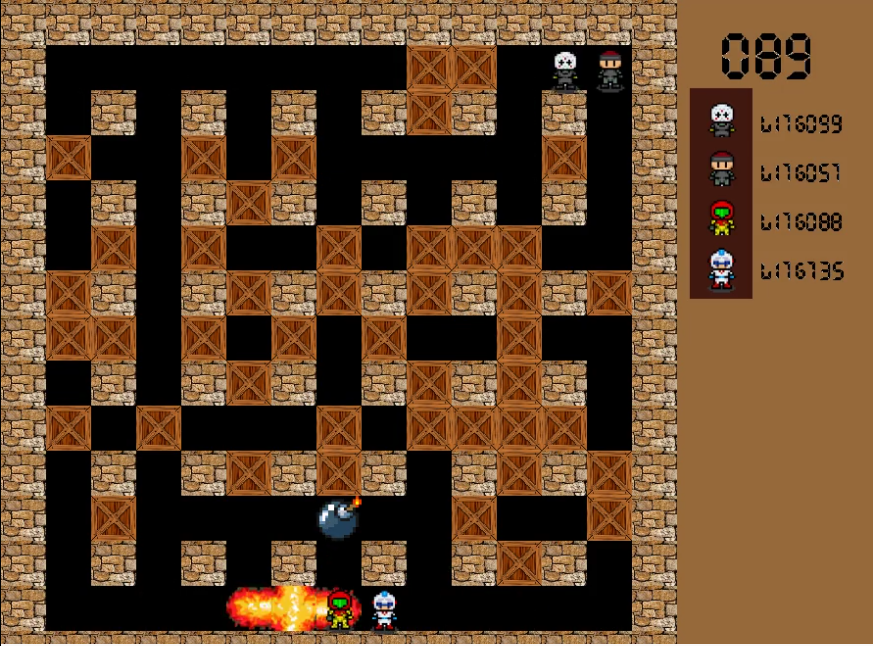
\includegraphics[scale=0.45]{sistemaFeedBack.jpg}
  \caption{Sistem de Feedback (\textbf{Bot 135}).}
  \label{img4:sistemaFeedback}
\end{figure}

\subsection{Testes da Sexta Tarefa}
Para a realização dos testes da Sexta Tarefa, utilizou-se o Sitema de Feedback, realizado pelos docentes, que coloca o \textbf{Bot} a competir com outros \textbf{Bots} de outros grupos de trabalho. Mas também testou-se através do \textbf{ghci}, as diversas situações que podem ocorrer com o \textbf{Bot}
%Adicionei este verbatim, para que a imagem do Sistema de FeedBack, venha antes da conclusão!
\begin{verbatim}





\end{verbatim}

\section{Conclusão}
\label{conclusao}
A realização deste projeto, propôs um grande desafio para o nosso grupo de trabalho tornando-se muito enriquecedor, pois desenvolvemos o raciocínio lógico e os métodos de trabalho.

Terminado este trabalho, alcançou-se o objectivo inicial do projeto. 

No decorrer do mesmo surgiram algumas dificuldades, como a manipulação de Strings e a determinação das condições a testar em cada Tarefa, dificuldades essas que se foram dissipando, com aplicação dos conteúdos programáticos abordados nas aulas teóricas e o apoio indespensável dos docentes, como forma a ultrapassar e resolver todos os problemas surgidos.

Sugerimos assim, a continuidade da realização destes projetos, como forma a desensolver espírito criativo e funcional indespensável à prática da nossa Profissão. 

\end{document}